\section{Perspektywa wariantów użycia systemu}

\subsection{Diagram wariantów użycia systemu}

\begin{figure}[H]
    \centering
    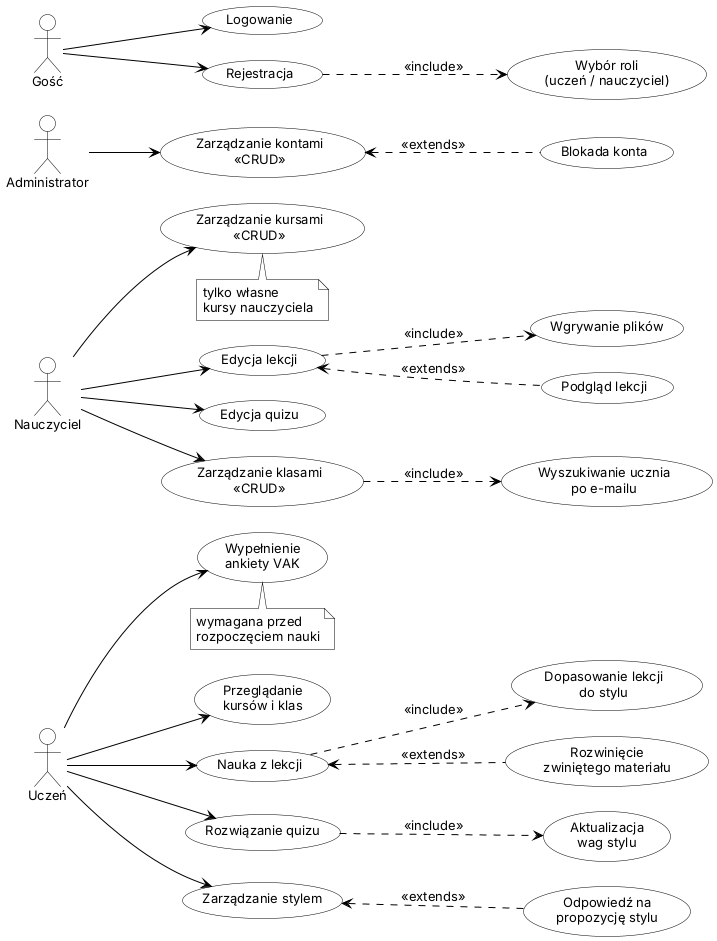
\includegraphics[width=0.85\linewidth]{images/use-cases.png}
    \caption{Diagram przypadków użycia systemu}
\end{figure}

\subsection{Opisy tekstowe aktorów}

\begin{itemize}[leftmargin=*]
    \item \textbf{Gość} -- osoba niezalogowana. Widzi stronę startową z opisem systemu, może założyć konto (jako uczeń albo nauczyciel) lub zalogować się.

    \item \textbf{Uczeń} -- zalogowany użytkownik, który się uczy. Przed rozpoczęciem nauki musi wypełnić ankietę VAK. Ma dostęp do kursów opublikowanych oraz kursów przypisanych do jego klas, uczy się z lekcji dopasowanych do swojego stylu, rozwiązuje quizy i zarządza swoim stylem uczenia się.

    \item \textbf{Nauczyciel} -- tworzy i edytuje własne kursy, lekcje, materiały i quizy, publikuje kursy oraz prowadzi klasy, do których dodaje uczniów i przypisuje kursy.

    \item \textbf{Administrator} -- zarządza kontami nauczycieli i uczniów: tworzy je, edytuje i blokuje. Konto administratora tworzy się poleceniem w konsoli, nie przez rejestrację.
\end{itemize}

\subsection{Opisy tekstowe wariantów użycia}

\subsubsection{Rejestracja}
\textbf{Numer:} UC-01 \quad \textbf{Aktor:} Gość

\textbf{Krótki opis:} Założenie konta ucznia albo nauczyciela. Rola jest wybierana przy rejestracji i nie zmienia się później.

\textbf{Główny przepływ zdarzeń:}
\begin{enumerate}[leftmargin=*]
    \item Gość klika ,,Załóż konto'' na stronie startowej
    \item Gość wybiera rolę (Uczeń / Nauczyciel), podaje imię, e-mail i hasło (min. 8 znaków)
    \item System sprawdza dane i unikalność adresu e-mail
    \item System tworzy konto, rozpoczyna sesję i przekierowuje do panelu użytkownika
\end{enumerate}

\subsubsection{Logowanie}
\textbf{Numer:} UC-02 \quad \textbf{Aktor:} Gość

\textbf{Krótki opis:} Zalogowanie się adresem e-mail i hasłem.

\textbf{Główny przepływ zdarzeń:}
\begin{enumerate}[leftmargin=*]
    \item Gość klika ,,Zaloguj się'' i podaje e-mail oraz hasło
    \item System weryfikuje dane oraz to, czy konto nie jest zablokowane
    \item System zapisuje sesję w ciasteczku i przekierowuje do panelu użytkownika
\end{enumerate}

\subsubsection{Wypełnienie ankiety VAK}
\textbf{Numer:} UC-03 \quad \textbf{Aktor:} Uczeń

\textbf{Krótki opis:} Ankieta wyznacza styl uczenia się ucznia i startowe wagi form V, A, K. Uczeń bez ankiety jest na nią kierowany z każdej strony systemu.

\textbf{Główny przepływ zdarzeń:}
\begin{enumerate}[leftmargin=*]
    \item System przekierowuje ucznia bez ankiety na stronę ankiety
    \item Uczeń odpowiada na 20 pytań (każda odpowiedź odpowiada jednej formie)
    \item System zlicza punkty V, A, K i wyznacza styl (forma lub formy z największą liczbą punktów)
    \item System zapisuje wynik oraz profil ucznia i wyświetla styl z punktami na wykresie
\end{enumerate}

\subsubsection{Przeglądanie kursów i klas}
\textbf{Numer:} UC-04 \quad \textbf{Aktor:} Uczeń

\textbf{Krótki opis:} Uczeń przegląda katalog kursów opublikowanych oraz swoje klasy z przypisanymi kursami.

\textbf{Główny przepływ zdarzeń:}
\begin{enumerate}[leftmargin=*]
    \item Uczeń wybiera ,,Kursy'' -- system wyświetla kursy opublikowane
    \item Uczeń wybiera ,,Moje klasy'' -- system wyświetla klasy ucznia z nauczycielem i liczbą kursów
    \item Uczeń otwiera kurs -- system wyświetla wstęp i listę lekcji
\end{enumerate}

\subsubsection{Nauka z lekcji}
\textbf{Numer:} UC-05 \quad \textbf{Aktor:} Uczeń

\textbf{Krótki opis:} Uczeń otwiera lekcję podaną według swojego stylu i w razie potrzeby rozwija materiały innych stylów.

\textbf{Główny przepływ zdarzeń:}
\begin{enumerate}[leftmargin=*]
    \item Uczeń otwiera lekcję z listy lekcji kursu
    \item System wyświetla bloki w kolejności nauczyciela; załączniki form spoza stylu ucznia są zwinięte
    \item System wyświetla uzasadnienie ,,dlaczego to widzisz'' i liczbę zwiniętych materiałów
    \item Uczeń może kliknąć ,,Pokaż materiał'' -- system rozwija materiał i zapamiętuje jego formy w stylu efektywnym lekcji
\end{enumerate}

\subsubsection{Rozwiązanie quizu}
\textbf{Numer:} UC-06 \quad \textbf{Aktor:} Uczeń

\textbf{Krótki opis:} Uczeń rozwiązuje quiz na końcu lekcji; system ocenia wynik i aktualizuje wagi stylu ($<<$include$>>$ Aktualizacja wag stylu).

\textbf{Główny przepływ zdarzeń:}
\begin{enumerate}[leftmargin=*]
    \item System wyświetla pytania wspólne i pytania o materiały form stylu efektywnego
    \item Uczeń zaznacza odpowiedzi i klika ,,Sprawdź odpowiedzi''
    \item System ocenia odpowiedzi; wynik co najmniej 70\% oznacza zaliczenie
    \item System aktualizuje wagi form (pierwszy sukces i pierwsza porażka w lekcji)
    \item System wyświetla poprawne odpowiedzi, wynik i informację o zmianie wag
\end{enumerate}

\subsubsection{Zarządzanie stylem}
\textbf{Numer:} UC-07 \quad \textbf{Aktor:} Uczeń

\textbf{Krótki opis:} Uczeń przegląda swój styl i wagi, zmienia styl ręcznie lub odpowiada na propozycję zmiany stylu.

\textbf{Główny przepływ zdarzeń:}
\begin{enumerate}[leftmargin=*]
    \item Uczeń wybiera ,,Mój styl'' -- system wyświetla styl, jego źródło, wagi i historię ankiet
    \item Jeśli system ma propozycję, wyświetla baner z uzasadnieniem
    \item Uczeń klika ,,Przełącz'' (styl zmienia się na proponowany) albo ,,Zostaję przy swoim''
    \item Uczeń może też ręcznie wybrać styl, wrócić do stylu z ankiety lub wypełnić ankietę ponownie
\end{enumerate}

\subsubsection{Zarządzanie kursami}
\textbf{Numer:} UC-08 \quad \textbf{Aktor:} Nauczyciel

\textbf{Krótki opis:} Nauczyciel tworzy i edytuje swoje kursy i lekcje oraz decyduje o publikacji.

\textbf{Główny przepływ zdarzeń:}
\begin{enumerate}[leftmargin=*]
    \item Nauczyciel wybiera ,,Moje kursy'' i klika ,,Nowy kurs''
    \item Nauczyciel podaje tytuł i opis; system tworzy kurs prywatny
    \item Nauczyciel uzupełnia wstęp, dodaje lekcje i ustala ich kolejność
    \item Nauczyciel publikuje kurs -- kurs pojawia się w katalogu uczniów
\end{enumerate}

\subsubsection{Edycja lekcji}
\textbf{Numer:} UC-09 \quad \textbf{Aktor:} Nauczyciel

\textbf{Krótki opis:} Nauczyciel układa treść lekcji z bloków tekstu i załączników oznaczonych formami V, A, K.

\textbf{Główny przepływ zdarzeń:}
\begin{enumerate}[leftmargin=*]
    \item Nauczyciel otwiera lekcję w edytorze
    \item Nauczyciel dodaje blok tekstu (,,+ Tekst'') lub załącznik (,,+ Załącznik'')
    \item Przy załączniku wybiera typ, wgrywa plik lub podaje adres, wpisuje tytuł i zaznacza formy V/A/K
    \item Nauczyciel zmienia kolejność bloków i klika ,,Zapisz lekcję''
    \item System sprawdza poprawność bloków i plików oraz zapisuje lekcję
\end{enumerate}

\subsubsection{Edycja quizu}
\textbf{Numer:} UC-10 \quad \textbf{Aktor:} Nauczyciel

\textbf{Krótki opis:} Nauczyciel tworzy quiz na końcu lekcji.

\textbf{Główny przepływ zdarzeń:}
\begin{enumerate}[leftmargin=*]
    \item Nauczyciel w podglądzie lekcji klika ,,Dodaj quiz'' lub ,,Edytuj quiz''
    \item Nauczyciel dodaje pytania (3--4 odpowiedzi, jedna poprawna) i wskazuje, czy pytanie dotyczy materiału formy V, A lub K
    \item Nauczyciel klika ,,Zapisz quiz''; system sprawdza i zapisuje quiz
\end{enumerate}

\subsubsection{Zarządzanie klasami}
\textbf{Numer:} UC-11 \quad \textbf{Aktor:} Nauczyciel

\textbf{Krótki opis:} Nauczyciel tworzy klasy, dodaje do nich uczniów i przypisuje kursy (także prywatne).

\textbf{Główny przepływ zdarzeń:}
\begin{enumerate}[leftmargin=*]
    \item Nauczyciel wybiera ,,Klasy'' i tworzy nową klasę
    \item Nauczyciel klika ,,Dodaj ucznia'', wpisuje fragment e-maila i dodaje ucznia z wyników wyszukiwania
    \item Nauczyciel klika ,,Przypisz kurs'' i wybiera swój kurs
    \item Uczniowie klasy widzą przypisane kursy w ,,Moich klasach''
\end{enumerate}

\subsubsection{Zarządzanie kontami}
\textbf{Numer:} UC-12 \quad \textbf{Aktor:} Administrator

\textbf{Krótki opis:} Administrator zarządza kontami nauczycieli i uczniów.

\textbf{Główny przepływ zdarzeń:}
\begin{enumerate}[leftmargin=*]
    \item Administrator wybiera ,,Użytkownicy'' i zakładkę Nauczyciele lub Uczniowie
    \item Administrator dodaje konto (imię, e-mail, hasło) lub edytuje istniejące
    \item Administrator może zablokować konto -- zablokowany użytkownik nie zaloguje się
\end{enumerate}

\subsection{Przykładowe diagramy sekwencji}

\subsubsection{Przykład 1. Pierwsze logowanie ucznia i ankieta VAK}

\begin{figure}[H]
    \centering
    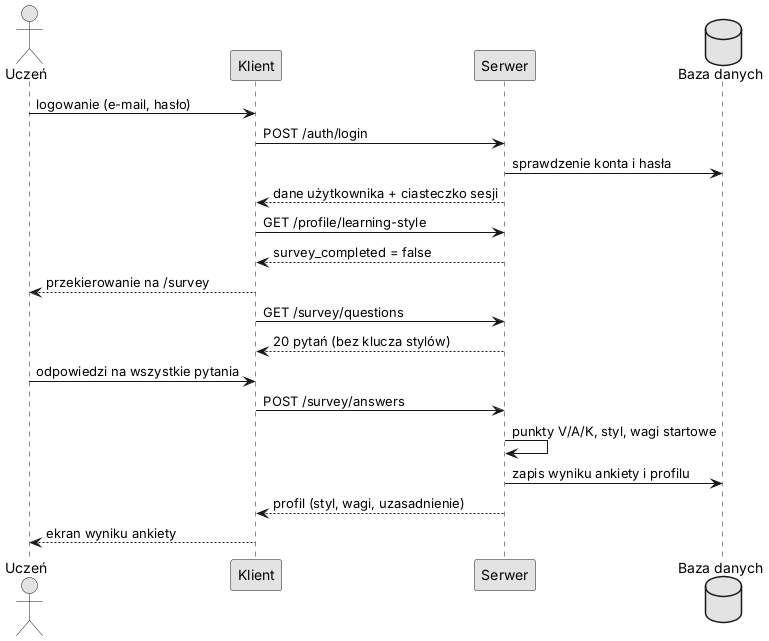
\includegraphics[width=0.85\linewidth]{images/seq-survey.png}
\end{figure}

Uczeń bez wypełnionej ankiety loguje się do systemu. Klient pobiera profil ucznia, a ponieważ ankieta nie została wypełniona, przekierowuje ucznia na stronę ankiety. Pytania przychodzą bez informacji, której formie odpowiada dana odpowiedź -- punkty liczy serwer. Po wysłaniu odpowiedzi serwer wyznacza styl i wagi startowe, zapisuje wynik i profil, a uczeń widzi ekran z wynikiem.

\subsubsection{Przykład 2. Lekcja dopasowana do stylu i rozwinięcie materiału}

\begin{figure}[H]
    \centering
    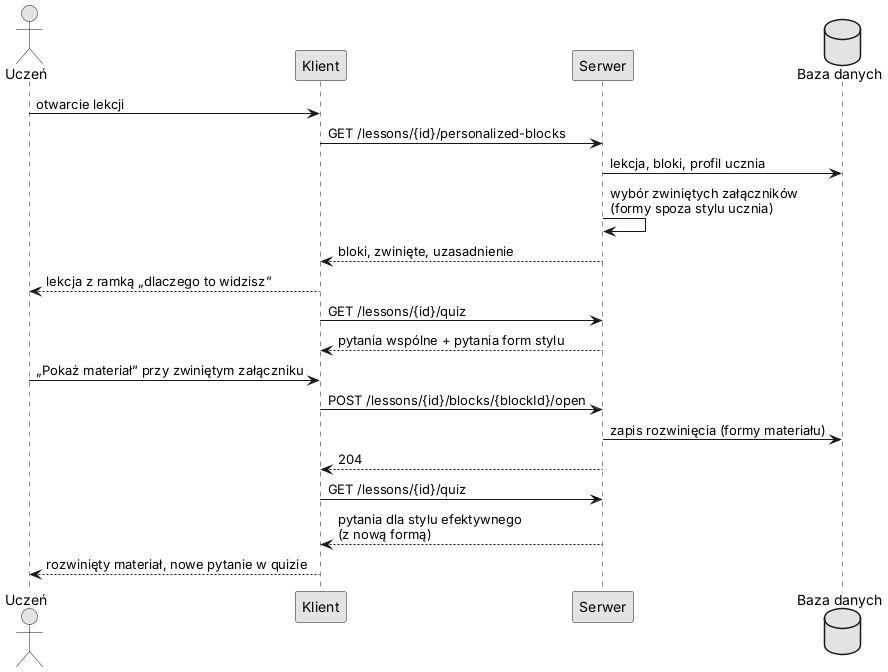
\includegraphics[width=0.85\linewidth]{images/seq-lesson.png}
\end{figure}

Serwer zwraca wszystkie bloki lekcji wraz z listą załączników do zwinięcia (tych, których żadna forma nie należy do stylu ucznia) oraz uzasadnieniem. Gdy uczeń rozwija zwinięty materiał, serwer zapisuje to zdarzenie, a formy materiału trafiają do stylu efektywnego lekcji. Klient pobiera quiz ponownie -- pojawia się w nim pytanie o materiał nowej formy.

\subsubsection{Przykład 3. Rozwiązanie quizu i adaptacja}

\begin{figure}[H]
    \centering
    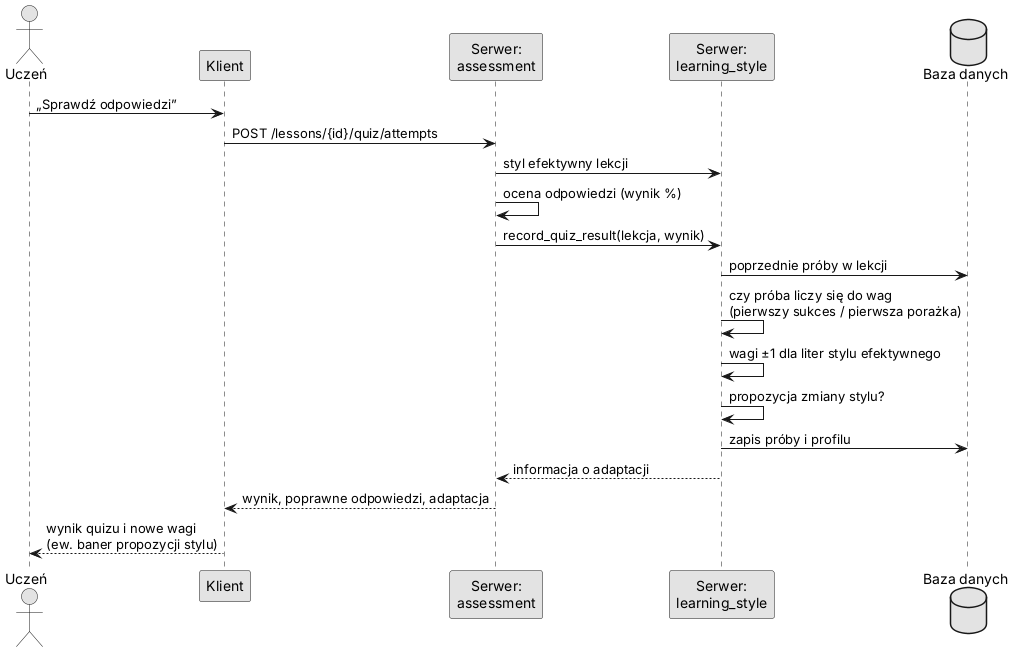
\includegraphics[width=0.85\linewidth]{images/seq-quiz.png}
\end{figure}

Moduł \texttt{assessment} ocenia odpowiedzi wyłącznie po stronie serwera i przekazuje wynik do modułu \texttt{learning\_style} przez jedną funkcję \texttt{record\_quiz\_result}. Moduł stylu sprawdza, czy próba liczy się do wag, zmienia wagi liter stylu efektywnego o $\pm 1$ i sprawdza, czy należy zaproponować zmianę stylu. Uczeń widzi wynik, poprawne odpowiedzi i informację o adaptacji.